\section{Design Pattern - Observer}
\label{sec:observer}

% Não remover a \ que vem a seguir à ", pois se for removida o espaço que vem a seguir desaparece no pdf
\hspace{5mm} O design pattern \textbf{Observer} implementa "uma para muitas"\ dependências, isto é, um objecto ("\textit{the subject}") "observado"\ por vários objectos observadores/dependentes (\textit{"observers"}). Desta forma, todos os \textit{observers} são automaticamente notificados, quando o \textit{subject} modifica o seu estado.

\begin{figure}[H]
    \centering
    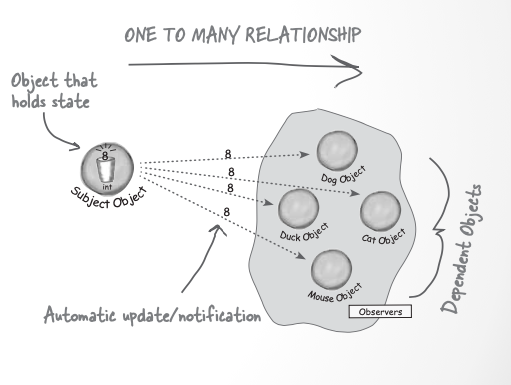
\includegraphics[scale=0.55]{images/observer-1.png}
    \caption{Ilustração do design pattern Observer.}
    \label{fig:mod_dom}
\end{figure}

\hspace{2mm} O \textit{subject} contém o \textit{data model} (\textit{state}) e/ou lógica de negócio, por outro lado, delega-se as funcionalidades da \textit{view} para os \textit{observers}. Desta forma, percebe-se que este design pattern pode ser usado em \textbf{MVC} (Model-View-Controller), no entanto, pode ser aplicado a outras situações.


\begin{figure}[H]
    \centering
    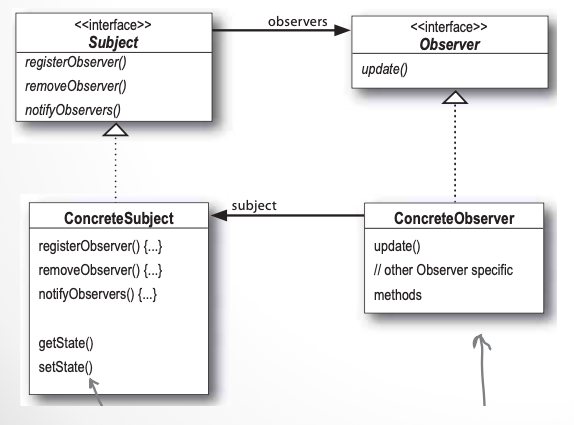
\includegraphics[scale=0.55]{images/observer-2.png}
    \caption{Arquitetura do design pattern Observer.}
    \label{fig:diagrama-classes-observer}
\end{figure}


\hspace{2mm} Os próprios \textit{observers} registam-se como observadores do \textit{subject}, quando têm interesse em serem notificados após uma alteração do estado deste, ou removem-se para deixar de receber essas notificações. 

\hspace{2mm} Com a finalidade de reutilização deste \textit{design pattern}, para diferentes \textit{subjects}, o mesmo sugere a criação de duas interfaces denominadas \textbf{Subject} e \textbf{Observer}, que delegam os métodos necessários para a concretização deste design pattern. Assim, para utilização deste design pattern, as classes observadas e observadoras devem implementar estas interfaces respetivamente. 

\hspace{2mm} Desta forma, e como foi dito anteriormente os \textit{observers} registam-se/removem-se do subject, logo este comportamento irá ser definido no \textbf{ConcreteSubject}, classe que implementa a interface \textbf{Subject}, mas para ser usado/chamado na classe \textbf{ConcreteObserver}, classe essa, que implementa a interface \textbf{Observer}. Isto significa que, a \textbf{ConcreteObserver} vai ser composta por uma variável de instância do tipo \textbf{Subject}/\textbf{ConcreteSubject} (mais adiante perceber-se-á a razão de existir a opção de ser dos dois tipos), denominada na figura \ref{fig:diagrama-classes-observer} por \textbf{subject}, para registar o \textit{observer} no \textit{subject} (registar o \textit{observer}, consiste adicioná-lo a uma estrutura de dados definida na \textbf{ConcreteSubject}, explicada mais adiante). Ainda na classe \textbf{ConcreteObserver} define-se o método \textbf{update}, que será chamado quando o \textit{subject} necessitar de notificar o \textit{observer} e através deste enviar dados importantes para esta notificação.

\hspace{2mm} Por outro lado, a classe \textbf{ConcreteSubject} vai ser constituída por uma estrutura de dados (p.e. \textit{Collection}), que aglomere os observadores desse \textit{subject}. Nesta classe, para além dos métodos de registo e remoção de observadores referidos anteriormente, existe ainda o método \textbf{notifyObservers}, que tal como o nome sugere, notificará os observadores, quando o estado do \textit{subject} (\textbf{ConcreteSubject}) se alterar. O \textbf{notifyObservers} percorre a estrutura de dados que aglomera os \textit{observers}, invocando o método \textbf{update}, definido nos mesmos, enviando os dados necessários.

\hspace{2mm} Neste design pattern, verifica-se ainda uma das grandes vantagens do mesmo, que consiste na redução de dependências entre as classes concretas, que muitas vezes impedem a evolução do código. Desta forma, a classe \textbf{ConcreteSubject}, não depende da classe \textbf{ConcreteObserver} e vice versa, pois apenas conhecem/dependem das interfaces \textbf{Subject} e \textbf{Observer}. 

\hspace{2mm} Na verdade, poder-se-á pensar que o que foi afirmado antes, não é verdade, visto que na figura \ref{fig:diagrama-classes-observer}, existe uma dependência clara do \textbf{ConcreteObserver}, em relação ao \textbf{ConcreteSubject}. Realmente, esta dependência poderá acontecer, com o objectivo de facilitar o \textit{observer} a aceder ao estado do \textit{subject}. No entanto, como já se referiu anteriormente, podem ser enviados valores através do método \textbf{update}, e assim, não ser necessário criar esta dependência. Por outro lado, pode-se pensar que ao enviar dados pelo método \textbf{update}, este terá que ser específico a cada problema, e não se poderá reutilizar a interface \textbf{Observer}. No entanto, para resolver facilmente esta situação, coloca-se um argumento nos métodos \textbf{notifyObservers} e \textbf{update} do tipo \textbf{Object}, ou seja, pode-se enviar objectos de qualquer tipo, pois por exemplo na linaguagem \textit{Java}, todo o objecto é do tipo \textbf{Object}.

\hspace{5mm} Ainda, torna-se importante realçar, o facto de poder-se ter diferentes objectos observadores para o mesmo objecto observado. Quando diz-se diferentes, quer-se dizer, classes diferentes, no entanto, implementam a mesma interface, tornando-os do mesmo tipo. Assim, com esta vantagem torna-se possível por exemplo, de forma estruturada e organizada, ter um sensor de temperatura, classe observada, e diferentes formas de apresentação, classes observadoras (graus Celsius e Fahrenheit). Em relação ao exemplo prático apresentado em anexo \ref{anexo:observer}, apenas foi desenvolvida a classe \textbf{ConcreteObserver}, mas poderiam ter sido elaboradas diferentes classes que implementassem o \textbf{Observer} e apresentassem a informação de forma diferente.

\hspace{5mm} A linguagem \textit{Java} tem diversos design patterns implementados, e o \textbf{Observer} não é excepção, tendo este diversas implementações. Uma das primeiras, senão a primeira versão de implementação deste design pattern na ferramenta, não foi bem conseguida, sendo isso reconhecido pela própria equipa do \textit{Java}, tornando a classe em questão \textit{deprecated}. A classe denomina-se por \textbf{Observable}, que "corresponde"\ ao \textbf{Subject} no caso apresentado acima. Desta forma, recomenda-se a não utilização do \textbf{Observable}, e fazer a interface \textbf{Subject} ou procurar por melhores alternativas, tais como \textbf{Listeners}.

%\hspace{5mm} A classe em questão denomina-se por \textbf{Observable}, que "corresponde"\ ao \textbf{Subject} no caso apresentado acima (as aspas devem-se ao facto do \textbf{Observable} ser uma classe e o \textbf{Subject} uma interface, logo não deveriam corresponder, mas mais adiante perceber-se-á). O problema desta classe, começa por isso mesmo, por ser uma classe, obrigando os utilizadores, a necessitarem de estender esta classe para a poderem usar, e como em \textit{Java} apenas se pode estender uma classe, significa que impede estender mais classes, ou estender o \textbf{Observable}, por já estar a estender outra classe. No entanto, o problema de ser classe poderia ser facilmente contornado, o que torna esta implementação má, consiste na colocação de alguns métodos \textit{protected}, ou seja, significa que os mesmos não podem ser usados por composição, dificultando a utilização do design pattern. Desta forma, recomenda-se a não utilização do \textbf{Observable}, e fazer a interface \textbf{Subject} ou procurar por melhores alternativas. 

\hspace{5mm} Por outro lado, o \textit{Java} definiu a interface \textbf{Observer}, não contendo qualquer problema, recomendando-se a sua utilização (no exemplo prático, definiu-se o \textbf{Observer}, mas poderia ter sido utilizado o do \textit{Java}).

\hspace{2mm} Em anexo \ref{anexo:observer}, apresenta-se um exemplo prático da aplicação deste design pattern. Utilizou-se, para facilitar a interpretação, os mesmos nomes para as classes e variáveis de instância da figura \ref{fig:diagrama-classes-observer}.